% !TEX root = ../main.tex

\chapter{量子淬火动力学中的普适临界现象}

	本章我们将证明在量子多体系统中,基态所对应的量子临界点也能够控制远离平衡态的动力学普适行为。
	这种普适行为体现在系统的量子几何的演化上。
	通过研究二次型格点费米子系统的量子淬火动力学,我们证明了系统的量子态体积通常随时间呈现线性增长, 并且线性增长率展现出了普适的规律:它的一阶导数随着控制参数的变化在量子临界点两侧出现跳变。
	这个跳变值和系统的的绝大部分细节信息无关,只被系统的维度所决定。
	这个结果揭示了非平衡量子多体系统存在普适的动力学性质。

	\section{研究背景}
	
		在量子多体系统中,量子相变是一个很重要的概念。
		与经典相变不同,它由量子涨落而非热运动驱动,并且在系统的基态上会表现出非解析行为。
		尽管在现实世界中,物质不可能被冷却到绝对零度,也就无法到达真正的基态,但低能激发态仍然会受到量子临界点的影响。
		如果我们观察量子相变的相图,就会发现在相图上呈现出一个V字形的,从量子相变点向有限温度展开的量子临界区域~\cite{Sachdev1999}。
		也就是说,量子临界性并不是一个仅存在于在理论的概念,而是一个切实存在的现象,是它决定了量子临界材料的有限温特性~\cite{Coleman2005}。
		迄今为止,大多数研究都集中在量子临界系统的热平衡特性上,而人们对于量子临界性的非平衡特性则了解甚少~\cite{Torre2010}。
		这是驱动我们开展本章研究的一个重要原因。
		
		非平衡物理通常比平衡态物理更为复杂和丰富,现实生活中的很多现象也都是非平衡的现象。
		在量子临界性方面,人们已经做出了大量努力来探索量子临界点附近的普适动力学行为。
		这其中包括量子临界点处的普适弛豫~\cite{Sachdev1997}以及由Kibble-Zurek机制~\cite{Kibble1976,Zurek1985} 控制的扫描动力学~\cite{Zurek2005,Dziarmaga2005,Damski2005}等。
		尽管这些现象和非平衡相关,但它们只涉及位于临界点上方的低能激发态,因此与基态本身的量子临界点有着根本联系。
		相比于这些“近平衡动力学”,量子临界性的作用在远离基态的系统中仍然没有被研究清楚。
		值得一提的是,最近的研究进展表明,在长程相互作用系统的量子淬火动力学中存在着本征的非平衡临界标度~\cite{Titum2020,De2023}。
		本章我们将揭示,即使在像二次型自由费米子这样简单的系统中,基态的量子相变也会导致远离基态的动力学中出现普适的非解析行为,而这种行为可以通过量子几何来刻画。
		
		人们引入了量子几何的概念最初是为了度量量子态之间的距离。
		它包含了两个部分的信息,一个是由贝里曲率~\cite{Bohm2003}表征的相位距离,另一个是由量子度规~\cite{Provost1980,Matsuura2010,Ma2010b}表征的幅值距离。
		相比而言,在过去的几十年里贝里曲率在拓扑物理学背景下已经被深入研究,而量子度规直到最近才受到关注。
		从实验方面来说,量子度规已经在各种人工量子系统中被测量和研究,包括冷原子~\cite{Yi2023}、氮空位中心~\cite{Yu2019} 和超导电路~\cite{Zheng2022}等实验。
		现在人们已经认识到,从平带超导和超流\cite{Peotta2015,Julku2016,Peotta2023,Tian2023,Espinosa2024} 到反常霍尔效应~\cite{Gianfrate2020,Wang2021,Gao2023}、 量子Fisher信息~\cite{Braunstein1994,Zanardi2007,Hauke2016}、电子-声子相互作用~\cite{Yu2023} 以及分数量子霍尔绝缘体\cite{Parameswaran2013,Neupert2015,BMera2021,BMera20212},包括量子度规在内的整个量子几何深刻地影响着多种多样的现象~\cite{Torma2023}。
		在量子相变的背景下,量子几何也已经被研究过~\cite{CAROLLO20201}。
		本章我们将揭示量子度规在解释量子系统中的非平衡现象,特别是在远离基态的临界动力学中的关键作用。

	\section{模型与研究方法}
	
		\subsection{模型介绍}
	
			为了研究更有一般性,我们选取了具有空间平移不变性的二次型费米子模型,经过傅里叶变换之后,其动量空间的哈密顿量可以一般地表示为:
			\begin{equation}
				H=\sum_k C^\dagger_k \hat{\mathcal{H}}_k C_k, \label{eq:Ham}
			\end{equation}
			其中每个动量模式下,最简单的情况就是$\hat{\mathcal{H}}_k$的维度为2的情形,即二能级系统,也是本章中我们聚焦的情形。
			2$\times$2的矩阵可以用泡利矩阵和单位阵进行正交分解,以方便后续计算,分解后一共有4个分量。
			由于单位阵对应的分量只影响系统能量的绝对值,不影响系统的其他物理行为,我们就可以假设该分量为0。
			于是我们将哈密顿量分解为$\hat{\mathcal{H}}_k = \vec{h}_k \cdot \vec{\sigma}$,其中$\vec{\sigma} = [\hat{\sigma}^X, \hat{\sigma}^Y, \hat{\sigma}^Z]$代表泡利矩阵,而$\vec{h}_k = [h_k^X, h_k^Y, h_k^Z]$是三分量的矢量,以下称“哈密顿矢量”。
			另一方面,生成和湮灭算符$C_k$和$C^\dagger_k$既可以表记两分量的费米子$C_k = [c_{\alpha, k}, c_{\beta, k}]^\text{T}$(其中$\alpha, \beta$可以代表子格、 轨道或者自旋的自由度),又可以表记南部表象$C_k = [c_k, c_{-k}^\dagger]^\text{T}$,它描述的是具有配对相互作用的费米子模型。
			系统的色散关系为$\epsilon_k^{\pm} = \pm \lvert \vec{h}_k \rvert$,上下两个能带之间的能隙为$\Delta_k = 2\lvert \vec{h}_k \rvert$。
			这样的二次型费米子模型中的量子相变一般由一个或多个能隙闭合点处$\Delta_k$的非解析行为所决定。
			当$\Delta_k$趋于0时, $\hat{\mathcal{H}}_k$趋于全零矩阵, 这引发了波函数乃至大部分可观测物理量的非解析行为。
			
			$\hat{\mathcal{H}}_k$在量子相变点处的非解析行为不仅影响了系统的定态性质比如基态能量, 对远离基态的动力学也有显著的影响。
			为了阐述这一论点,我们研究了已经在可积系统中被广泛研究过~\cite{Barthel2008,Calabrese2011,Mitra2018}的量子淬火动力学。
			在量子淬火动力学中,淬火操作一般会使得系统的波函数投影到新哈密顿量不同的能级上,通常平均来说是远离基态的。
			和之前的研究不同的是,我们将从另一个角度——量子几何的角度来研究这个问题。
			公式~\eqref{eq:Ham}中所给出的哈密顿量是由一系列解耦的动量模式所描述的二能级系统,其近动模式频率由能隙$\Delta_k$所决定。
			因此,$\Delta_k$的奇异性决定了系统的动力学, 且可以用量子几何的演化来刻画。
			我们将通过研究系统量子态体积的淬火动力学,来研究量子相变点处的非解析行为对远离基态的动力学的影响。
		
		\subsection{量子度规与量子态体积}
		
			量子度规可以用来衡量临近动量模式波函数之间的距离。
			考虑两个相差很小的动量模式所对应的波函数$|u^0_k\rangle$和$|u^0_{k+dk}\rangle$,由于近动频率的细微差别,它们在经过一段时间的演化之后会体现出差距。
			这两个态之间的距离可以用Fubini-Study度规$\mathbb{B}(k)$来刻画:
			\begin{equation}
				\mathbb{B}_{ij}(\mathbf{k})=\langle\partial_i \psi_\mathbf{k} |\partial_j \psi_\mathbf{k}\rangle-\langle\partial_i \psi_\mathbf{k} |\psi_\mathbf{k}\rangle \langle \psi_\mathbf{k}|\partial_j \psi_\mathbf{k}\rangle, \label{eq:metric}
			\end{equation}
			其中$\partial_i=\frac{\partial}{\partial k_i}$, $i=x,y$,而$|\psi_\mathbf{k}\rangle$是动量$\mathbf{k}$所对应的波函数。
			对于二维系统来说,Fubini-Study度规是一个$2\times2$的张量。
			$\mathbb{B}_{ij}(k)$的虚部部分是已经被广泛研究过的贝利相位,刻画的是随着$\mathbf{k}$的微小变化波函数的相位差别。
			而$\mathbb{B}_{ij}(k)$的实部部分是量子度规,度量的是两个动量差别很小的波函数之间的平行性,刻画的是希尔伯特空间里波函数矢量指向上的差距。
			为了衡量整个系统各个相邻动量波函数之间的差距,通过对整个布里渊区(BZ)进行积分,得到的是量子态体积(Quantum State Volume, QSV)~\cite{Ozawa20210},它也了刻画布里渊区中波函数所在流形的粗糙程度。
			对于二维系统,量子态体积$g$被定义为
			\begin{equation} \label{eq:g_2D}
				g_{2D}=\int d\mathbf{k} \sqrt{\det\Re[\mathbb{B}_{ij}(\mathbf{k})]},
			\end{equation}
			其中积分范围是第一布里渊区。
			只要给定了几何$\Re[\mathbb{B}]$,上述积分就是所谓的黎曼体积。
			它是规范不变的,所以是物理上可观测的希尔伯特空间的体积。
			而对于一维系统,公式~\eqref{eq:metric}约化为一个一维的张量(一个数):
			\begin{equation}\label{eq:B_1D}
				\mathbb{B}(k)= \langle \dot{\psi}_k|\dot{\psi}_k\rangle-\langle \dot{\psi}_k|\psi_k\rangle \langle \psi_k|\dot{\psi}_k \rangle,
			\end{equation}
			其中$\dot{u}_k=\partial u_k/\partial k$,以及一维的量子态体积为$g_{1D}=\int dk \sqrt{\mathbb{B}(k)}$。

	\section{研究结果}
	
		我们提出了一个广泛适用于二次型费米子系统淬火动力学的定理,不仅从解析上给出了证明,并且通过数值计算了不同的模型进行了检验。
		我们的主要结论是:对于一个具有空间平移不变性的、被一个控制参数$\lambda$所控制的哈密顿量$\hat{\mathcal{H}}_k(\lambda)$(见公式~\eqref{eq:Ham}),让系统初始时刻被制备在$\hat{\mathcal{H}}_k(\lambda_0)$的基态上,然后瞬间改变$\lambda$让系统在新的哈密顿量$\hat{\mathcal{H}}_k(\lambda_f)$下演化。
		如果$\lambda_f$恰好是系统能隙闭合的量子临界点,即$\lambda=\lambda_c$,那么系统量子态体积的时间演化就会展现出与系统的普适的临界动力学行为。
		这种普适的行为和系统的具体形式无关,与系统的绝大部分细节无关,只取决于系统的维度。
		在描述最关键的定理之前,我们先提出一个引理。
		
		\subsection{引理的阐述与证明}	
			{\bf 引理:}
			\textit{对于上述量子淬火动力学,系统的量子态体积通常呈现出线性增长(可能伴随着周期振荡),线性增长率依赖于$\lambda_f$。}
			
			我们可以这样理解这个结果:公式~\eqref{eq:metric}和\eqref{eq:B_1D}中量子度规的时间依赖来自波函数
			\begin{equation}\label{eq:phit}
				|\psi_k(t)\rangle=e^{-i\hat{\mathcal{H}}_k(\lambda_f)t}|\psi_k(0)\rangle
			\end{equation}
			所以公式~\eqref{eq:metric}和\eqref{eq:B_1D}对动量$k$的求导引入了量子态体积对时间$t$的线性依赖,这主导了量子态体积的长时动力学行为。		
			对于一维系统,我们可以证明:
			\begin{equation}\label{eq:Rk_1D}
				\mathbb{B}(k) = f_k^0(t)+f_k^1(t) t+R_k t^2. 
			\end{equation}
			其中$R_k$不依赖于时间$t$。
			
			下面我们推导一维系统量子态体积的长时动力学。
			为了得到公式~\eqref{eq:metric}的结果,我们对公式\eqref{eq:B_1D}关于$k$进行求导,得到
			\begin{equation}\label{eq:dphit}
				|\dot{\psi}_k(t)\rangle = (e^{-i\hat{\mathcal{H}}_k t})'|\psi_k(0)\rangle + 
				(e^{-i\hat{\mathcal{H}}_k t})|\dot{\psi}_k(0)\rangle
			\end{equation}
			其中$()'$也表示对$k$的导数,且方便起见表记上我们约定$\hat{\mathcal{H}}_k \equiv \hat{\mathcal{H}}_k(\lambda_f)$。
			由于我们关心的是长时动力学,且显然公式\eqref{eq:B_1D}中$t$的平方项来自波函数中$t$的一次项故我们可以对波函数及其导数只保留$t$的一次项。
			由于初态波函数不含时间,其对$k$的导数不贡献时间$t$的依赖,$t$的一次项完全来自时间演化算符对$k$求导所产生,于是公式\eqref{eq:dphit}约化为
			\begin{equation}\label{eq:dphit_reduced}
				|\dot{\psi}_k(t)\rangle = (e^{-i\hat{\mathcal{H}}_k t})'|\psi_k(0)\rangle
			\end{equation}
			为了方便对时间演化算符求导,我们先将哈密顿量进行对角化。
			引入哈密顿量对角化后的形式
			\begin{equation}\label{eq:diag}
				\hat{\mathcal{D}}_k = S_k^{-1} \hat{\mathcal{H}}_k S_k
			\end{equation}
			其中矩阵$S_k$是将哈密顿量对角化的正交阵,满足$S^{-1} = S^\dagger$,同时也依赖于$\lambda_f$。
			不难发现,对于二能级系统,对角化的哈密顿量直接和色散关系挂钩:
			\begin{equation}\label{eq:Dk}
				\hat{\mathcal{D}}_k = -\epsilon_k \hat{\sigma}_Z
			\end{equation}
			其中色散关系$\epsilon_k$约定为前文提到的上能带$\epsilon_k^+$。
			于是时间演化算符$e^{i\hat{\mathcal{H}}_k t}$也可以被$S_k$对角化:
			\begin{equation}
				e^{-i\hat{\mathcal{H}}_k t} = S_k e^{-i\hat{\mathcal{D}}_k t} S_k^{-1} = S_k e^{i\epsilon_k \hat{\sigma}_Z t} S_k^{-1}
			\end{equation}
			其对$k$求导的结果为
			\begin{equation}
				(e^{i\epsilon_k \hat{\sigma}_Z t})' = S_k (e^{i\epsilon_k \hat{\sigma}_Z t})' S_k^{-1} + S_k' e^{i\epsilon_k \hat{\sigma}_Z t} S_k^{-1} + S_k e^{i\epsilon_k \hat{\sigma}_Z t} (S_k^{-1})'
			\end{equation}
			保留时间$t$的一次项,得到
			\begin{equation}
				(e^{i\epsilon_k \hat{\sigma}_Z t})' = S_k (e^{i\epsilon_k \hat{\sigma}_Z t})' S_k^{-1} = i t \dot{\epsilon}_k S_k \hat{\sigma}_Z e^{i\epsilon_k \hat{\sigma}_Z t} S_k^{-1}
			\end{equation}
			于是公式\eqref{eq:dphit_reduced}可以被简化为
			\begin{equation}
				|\dot{\psi}_k(t)\rangle = i t \dot{\epsilon}_k S_k \hat{\sigma}_Z e^{i\epsilon_k \hat{\sigma}_Z t} S_k^{-1}|\psi_k(0)\rangle
			\end{equation}
			然后我们可以分别代入计算公式~\eqref{eq:metric}的两项。
			第一项为
			\begin{equation}
				\langle \dot{\psi}_k(t)|\dot{\psi}_k(t) \rangle = t^2 \dot{\epsilon}_k^2
			\end{equation}
			可以看出,这一项只包含淬火后哈密顿量的能谱信息,并不包含初态的信息。
			对于第二项,我们先算出
			\begin{equation}
				\langle \psi_k(t)|\dot{\psi}_k(t) \rangle = i t \dot{\epsilon}_k \langle \psi_k(0)|S_k \hat{\sigma}_Z S_k^{-1}|\psi_k(0) \rangle
			\end{equation}
			反过来利用公式\eqref{eq:diag}和\eqref{eq:Dk},我们就可以算出
			\begin{equation}
				\langle \psi_k(0)| S_k \hat{\sigma}_Z S_k^{-1} |\psi_k(0) \rangle= -\frac{\langle \psi_k(0)|\hat{\mathcal{H}}_k|\psi_k(0) \rangle}{\epsilon_k} = -\frac{\vec{h}_{0k}\cdot\vec{h}_{fk} }{\epsilon_{0k}\epsilon_k}
			\end{equation}
			于是第二项整体的结果为
			\begin{equation}
				\langle \dot{\psi}_k(t)|\psi_k(t) \rangle \langle \psi_k(t)|\dot{\psi}_k(t) \rangle = t^2 (\dot{\epsilon}_k)^2 \left(\frac{\vec{h}_{0k}\cdot\vec{h}_{fk}}{\epsilon_{0k}\epsilon_k}\right)^2
			\end{equation}
			最终我们得到了一维系统的$r_k$为
			\begin{equation} \label{Eq:rk_1D}
				r_k = \sqrt{R_k} = |\dot{\epsilon}_k|\sqrt{1-\left(\frac{\vec{h}_{0k}\cdot\vec{h}_{fk}}{\epsilon_{0k}\epsilon_k}\right)^2} = \frac{|{\vec{h}}_{0k}\times \vec{h}_{fk}||\dot{\epsilon}_k|}{|{\vec{h}}_{0k}|\cdot|\vec{h}_{fk}|},
			\end{equation}
			线性增长率为
			\begin{equation}\label{Eq:v_1D}
				v(\lambda_f) = \int dk r_k
			\end{equation}
			且$r_k$与时间无关,包含了初态的信息。
		
			对于二维系统,量子态体积的长时动力学的长时推导十分复杂,这里我们粗略地给出:
			\begin{equation}\label{eq:Rk}
				\det{\Re[\mathbb{B}_{ij}(\mathbf{k})]} = f_\mathbf{k}^0(t)+f_\mathbf{k}^1(t) t+R_\mathbf{k} t^2\sin^2[2 \epsilon_\mathbf{k} t]. 
			\end{equation}
			最后一项主导了$g_{2D}(t)$的长时动力学——伴随周期振荡的线性增长。
			将振荡项$|\sin2\epsilon_{\mathbf{k}}t|$用它在一个周期内的平均值$\frac 2\pi$代替之后,我们就得到$g_{2D}(t)\sim v(\lambda_f)t$。
			记$r_\mathbf{k} = \sqrt{R_{\mathbf{k}}}$,则线性增长率为
			\begin{equation}\label{Eq:v_2D}
				v(\lambda_f)=\frac 2\pi\int d\mathbf{k}r_\mathbf{k}
			\end{equation}
			且$r_{\mathbf{k}}$与时间无关,包含了初态的信息。
			
		\subsection{定理的阐述}
			
			{\bf 定理:}
			\textit{$v(\lambda_f)$关于$\lambda_f$的导数在量子临界点处展现出普适的跳变值:
				\begin{equation}\label{eq:Cd}
					\frac{dv}{d\lambda_f}\bigg |_{\lambda_f=\lambda_c^-} - \frac{dv}{d\lambda_f}\bigg |_{\lambda_f=\lambda_c^+} = \mathcal{N} C_d
				\end{equation}
				其中$\mathcal{N}$是第一布里渊区内的能隙闭合点个数,$C_d$代表了一个只跟系统维度有关的无量纲常数:
				\begin{eqnarray}\label{eq:cd}
					C_d = \left\{\begin{array}{cl}
						2\pi, & d=1;   \\
						8, & d=2. \\
					\end{array}\right.
				\end{eqnarray}
			}
		
			{\bf 假设条件:}
			上述定理的证明依赖于以下两点假设:
			\begin{enumerate}
				\item 哈密顿矢量${\vec{h}}_{\mathbf{k}}$的每个分量(即使是在量子临界点处)都是$\mathbf{k}$和 $\lambda$解析函数;
				\item 能隙闭合点是其邻域内的唯一极值点;
			\end{enumerate}
			事实上,绝大部分实际的物理模型都符合这两点假设。
			
			下一小节中我们将基于上述假设证明我们提出的定理。
			
		\subsection{定理的证明}
		
			我们的证明过程分为以下三步:
			\begin{enumerate}
				\item 第一步,我们证明了只有能隙闭合点$k_c$邻域内的动量模式对系统的非解析行为有贡献。这允许我们对哈密顿量在$k_c$附近进行泰勒展开,也是定理中与系统的特定形式无关的关键原因;
				\item 第二步,通过对泰勒展开后哈密顿量不同形式的分类和归并,简化了哈密顿矢量的形式;
				\item 第三步,基于第二步给出的简化形式证明$C_d$是一个普适的常数。
			\end{enumerate}
		
			% 插图
			\begin{figure}[!htp]
				\centering
				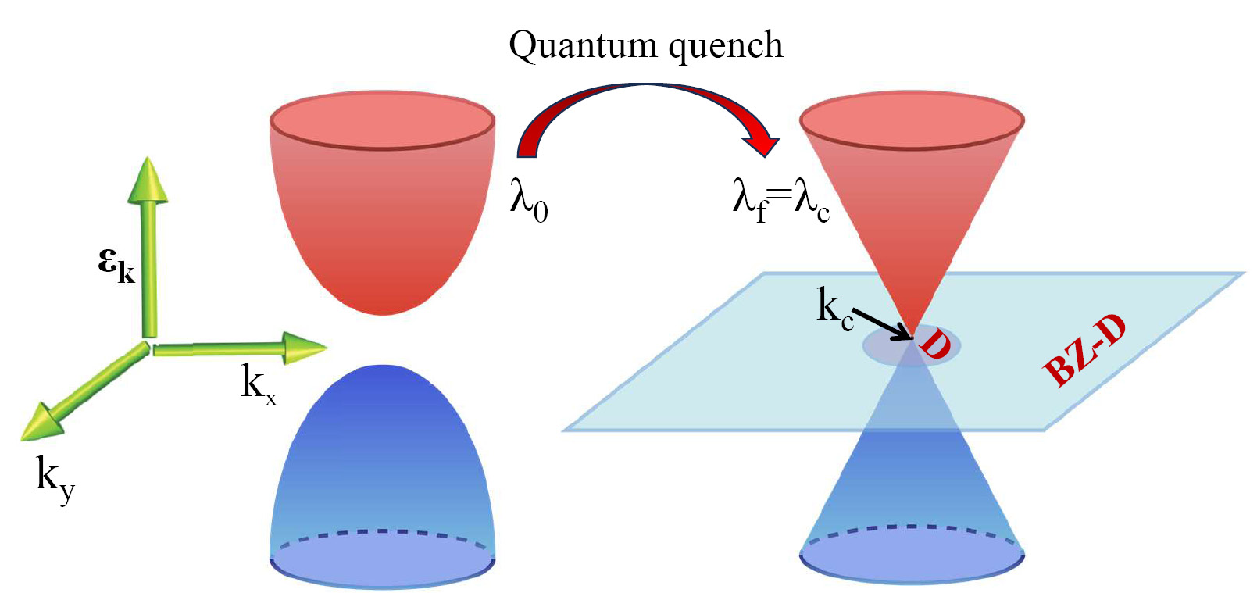
\includegraphics[width=0.9\textwidth]{figures/QV_BZ_D.pdf}
				\centering
				\bicaption{二维系统量子淬火动力学的示意图}{Illustration of the quantum quench dynamics in a 2D case} \label{Fig:BZ_D}
			\end{figure} 
		
		%\bicaption{二维系统量子淬火动力学的示意图。
			%阴影部分(区域$D$)表示了第一布里渊区中能隙闭合点$\mathbf{k}_c$附近的邻域。}{Illustration of the quantum quench dynamics in a 2D case.
			%The shadowed regime (denoted by $D$) indicates a small vicinity around the gap close point $\mathbf{k}_c$ in the 1st BZ.} \label{Fig:BZ_D}		
		
			{\bf 第一步:}
			哈密顿矢量${\vec{h}}_{\mathbf{k}}$的解析性允许我们将积分区间从整个第一布里渊区缩小到孤立能隙闭合点的邻域内。
			一般来说,对于任意的维度,公式\eqref{Eq:v_2D}和Eq.~\eqref{eq:Cd}的积分范围可以被缩小到第一布里渊区的一个开子集$S$,只要$S$包含了第一布里渊区的所有能隙闭合点,不管这些能隙闭合点是否是孤立的。
			简单起见,考虑第一布里渊区内只有一个能隙闭合点,我们需要证明:
			\begin{equation}\label{eq:BZ-D}
				\frac{d}{d\lambda_f} \int_{BZ-D} r_\mathbf{k}(\lambda_f) d\mathbf{k} \bigg|_{\lambda_f=\lambda_c^-} - \frac{d}{d\lambda_f} \int_{BZ-D} r_\mathbf{k}(\lambda_f) d\mathbf{k} \bigg|_{\lambda_f=\lambda_c^+}
			\end{equation}
			这一表达式为零。
			其中$D$是$\mathbf{k}_c$附近任意小的邻域。
			对于更高的维度,讨论的思路也是类似的。
			对于$D$关于第一布里渊区的补集$BZ-D$,$r_\mathbf{k}^2$是关于$\mathbf{k} \in BZ-D$和$\lambda \in (\lambda_c-\delta \lambda, \lambda_c+\delta \lambda)$双重解析的函数,所以$r_\mathbf{k} \sim \sqrt{R_\mathbf{k}}$和${\partial r_\mathbf{k}(\lambda_f)}/{\partial \lambda_f}$是有界的,于是关于$k$的积分和关于$\lambda_f$的导数可以交换:
			\begin{equation}
				\int_{BZ-D} \left(\frac{\partial r_\mathbf{k}(\lambda_f)}{\partial\lambda_f}  \bigg|_{\lambda_f = \lambda_c^-} - \frac{\partial r_\mathbf{k}(\lambda_f)}{\partial\lambda_f} \bigg|_{\lambda_f=\lambda_c^+}\right) d\mathbf{k}
			\end{equation}
			这部分贡献只能来自$R_\mathbf{k}(\lambda_c)$的零点,因为不解析性来自于对$R_\mathbf{k}(\lambda_c)$开根号。
			由于$R_\mathbf{k}(\lambda_c)$在$BZ-D$内是解析的且不恒为0,足以说明这些零点构成的是一个零测集,因此公式~\eqref{eq:BZ-D}的值为零。
			至此,我们得到了
			\begin{equation}
				\frac{d}{d\lambda_f} v(\lambda_f) \bigg|_{\lambda_f=\lambda_c^-} - \frac{d}{d\lambda_f} v(\lambda_f) \bigg|_{\lambda_f=\lambda_c^+}=\frac{d}{d\lambda_f} \tilde{v}(\lambda_f) \bigg|_{\lambda_f=\lambda_c^-} - \frac{d}{d\lambda_f} \tilde{v}(\lambda_f) \bigg|_{\lambda_f=\lambda_c^+},
			\end{equation}
			其中
			\begin{equation}\label{Eq:v_reduce}
				\tilde{v}(\lambda_f) \equiv \int_{D}{r_\mathbf{k}(\lambda_f) d\mathbf{k}},
			\end{equation}
			基于公式~\eqref{Eq:v_reduce},我们就可以对$r_\mathbf{k}$在能隙闭合点$k_c$附近进行泰勒展开,以简化后续计算。
			
			{\bf 第二步:}
			能隙闭合点的简单结构假设可以显著简化计算的过程。
			不失一般性地,我们可以通过$\mathbf{k}$和$\lambda_f$的变量代换使得$k_c=0$,$\lambda_c=0$。
			对于一维系统,我们对能隙闭合点的简单结构定义为:
			$\exists \delta \lambda, \forall \lambda \in (- \delta \lambda, \delta \lambda)$,使得$\epsilon_k^2$的泰勒展开满足:
			\begin{equation}
				\epsilon_k^2 = f(\lambda) k^{2n} + l(\lambda) + o(k^{2n}),
			\end{equation}
			其中$n$是$k$的最低次数,且
			\begin{equation}
				\begin{aligned}
					& \lim_{\lambda \rightarrow 0^-}{f(\lambda)} = \lim_{\lambda \rightarrow 0^+}{f(\lambda)} \equiv f(\lambda=0)\neq0,\\
					& \lim_{\lambda \rightarrow 0^-}{l(\lambda)} = \lim_{\lambda \rightarrow 0^+}{l(\lambda)} \equiv l(\lambda=0)=0.
				\end{aligned}
			\end{equation}
			这一条件意味着在泰勒展开的收敛域内,只要$k \neq k_c$或$\lambda \neq \lambda_c$,就有$\epsilon_k \neq 0$,而$\epsilon_k = 0$当且仅当$k=k_c$且$\lambda=\lambda_c$。
			这也排除了多个局域的极值点随着$\lambda$逼近$\lambda_c$收敛到同一个能隙闭合点的可能性。
			能隙闭合点简单结构的物理含义是明确的:$\lambda\rightarrow\lambda_c$时低能有效理论的形式是收敛的,这一点对于大量符合场论描述的格点模型都是成立的。
			哈密顿矢量${\vec{h}}_{\mathbf{k}}$的泰勒展开可以被一般地表示为
			\begin{equation}
				\vec{h}_k = [k^{n_X}(a_X \lambda + b_X) + o(k^{n_X}),
				k^{n_Y}(a_Y \lambda + b_Y) + o(k^{n_Y}),
				k^{n_Z}(a_Z \lambda + b_Z) + o(k^{n_Z})].
			\end{equation}
			既然当$\lambda=0$时,只要$k \neq 0$就有$\vec{h}_k \neq \mathbf{0}$,那么$\{n_X,n_Y,n_Z\}$这三个数中至少存在一个非零的数。
			于是下面我们进行分类讨论。
			\begin{enumerate}
				\item $\{n_X,n_Y,n_Z\}$中只有一个数为0。
				不失一般性地,通过SU$(2)$的基底变换,我们总能选取$n_Z=0$因此由于能隙在$\lambda_c = 0$处闭合所以$b_Z$必须为0。
				\begin{enumerate}
					\item 如果$n_X > n_Y$,那么对应的色散关系就是$\epsilon_k^2 \sim k^{2n_X}(a_X \lambda + b_X)^2 + k^{2n_Y}(a_Y \lambda + b_Y)^2 + \lambda^2$。(对于$n_X < n_Y$的讨论也是类似的。)
					\begin{enumerate}
						\item 如果$\epsilon_k^2$的主导项是拥有非零系数$(a_X\lambda+b_X)$的$k^{2n_X}$,那么必须要求$a_Y=b_Y=0$。
						不仅如此,$\sigma^Z$前面的高阶项必须被限制在$o(k^{2n_X})$。
						从简单结构假设出发还要求$b_X\neq0$。
						由于我们关心$\delta\lambda\ll1$的情况,于是我们可以忽略$a_X \lambda$。
						最后,哈密顿矢量可以被简化为$\vec{h}_k = [b_X k^{n_X} + o(k^{n_X}),0,\lambda + o(k^{2n_X})]$,其中$\lambda$的系数已经被归一化。
						\item 如果$\epsilon_k$的主导项是$k^{2n_Y}$,那么要求$b_Y \neq 0$,且出于和前一种情形同样的理由,$a_Y \lambda$可以被忽略。
						因此,哈密顿矢量可以被简化为$\vec{h}_k = [o(k^{n_Y}), b_Y k^{n_Y} + o(k^{n_Y}),\lambda + o(k^{2n_Y})]$。
					\end{enumerate}
					\item 如果$n_X = n_Y \ \dot= \ n$,那么通过一个SU$(2)$的基地变换,哈密顿矢量可以被简化为$\vec{h}_k = [\sqrt{b_X^2+c_Y^2} k^{n} + o(k^{n}), o(k^{n}),\lambda+ o(k^{2n})]$。
				\end{enumerate}
				\item $\{n_X,n_Y,n_Z\}$之中有两个数为0。
				不失一般性地,由于$\lambda_c = 0$我们可以假设$n_Y=n_Z=0$并且将$b_Y,b_Z$也设置为0。
				那么通过一个与$k$无关的基底变换,就可以得到哈密顿矢量的简化形式为$\vec{h}_k = [b_X k^{n_X} + o(k^{n_X}),0,\lambda + o(k^{2n_X})]$。
			\end{enumerate}
			总结以上的所有情况,我们可以得到$\vec{h}_k$的简化形式为:
			\begin{equation} \label{h_k_reduce_1D}
				\vec{h}_k = [J k^{n} + o(k^{n}), o(k^{n}), \lambda + o(k^{2n})].
			\end{equation}
		
			对于二维的系统,能隙闭合点的简单结构被定义为:
			当$\lambda \rightarrow \lambda_c$时,$\epsilon_\mathbf{k}^2$的泰勒展开形式可以被表示为
			\begin{equation}
				\epsilon_\mathbf{k}^2 = f_x(\lambda) k_x^\alpha + f_y(\lambda) k_y^\beta + g(\lambda) + o(k_x^\alpha) + o(k_y^\beta),
			\end{equation}
			其中$\alpha,\beta$是$k_x,k_y$的最低次数,且
			\begin{equation}
				\begin{aligned}
					& \lim_{\lambda \rightarrow \lambda_c^-}{f_{x(y)}(\lambda)} = \lim_{\lambda \rightarrow \lambda_c^+}{f_{x(y)}(\lambda)} \equiv f_{x(y)}(\lambda_c)\neq0,\\
					& \lim_{\lambda \rightarrow \lambda_c^-}{g(\lambda)} = \lim_{\lambda \rightarrow \lambda_c^+}{g(\lambda)} \equiv g(\lambda_c)=0.
				\end{aligned}
			\end{equation}
			和一维的情形类似,既然$\vec{h}_\mathbf{k}$中$k_x,k_y$的交叉项会对$\epsilon_\mathbf{k}$的收敛行为产生贡献,哈密顿矢量的泰勒展开通常可以被表示为
			\begin{equation}
				\vec{h}_\mathbf{k} = k_x^{\vec{\alpha}}(\vec{a} \lambda + \vec{b}) + k_y^{\vec{\beta}}(\vec{c} \lambda + \vec{d}) + o(k_x^{\vec{\alpha}} ,k_y^{\vec{\beta}}),
			\end{equation}
			类似地,$\{(\alpha_X,\beta_X),(\alpha_Y,\beta_Y),(\alpha_Z,\beta_Z)\}$之中至少有一个非零矢量。
			接下来我们进行分类讨论:
			\begin{enumerate}
				\item $\{(\alpha_X,\beta_X),(\alpha_Y,\beta_Y),(\alpha_Z,\beta_Z)\}$之中只有一个零矢量。
				不失一般性地,假设$\alpha_Z=0,\beta_Z=0$,且由于$\lambda_c = 0$我们可以将$b_Z,d_Z$设置为0。
				\begin{enumerate}
					\item 按照一维情况下的分析,如果$\alpha_X \neq \alpha_Y$,
					$k_x^{\alpha_X}(a_X \lambda + b_X)$和$k_x^{\alpha_Y}(a_Y \lambda + b_Y)$之中只有其中一项能被留下。
					然而,如果在这种情况下$k_x$和$k_y$出现在相同的泡利矩阵之前,那么$k_x,k_y$的交叉项就会进入$\epsilon_\mathbf{k}$的表达式,这和简单结构假设是矛盾的。
					于是哈密顿矢量的一种等价表示是$\vec{h}_\mathbf{k} = [k_x^{\alpha}(a_X \lambda + b_X) + o(k_x^{\alpha}, k_y^{\beta}),  k_y^{\beta}(c_Y \lambda + d_Y) + o(k_x^{\alpha}, k_y^{\beta}), \lambda + o(k_x^{2\alpha}, k_y^{2\beta})]$。
					对于$\beta_X \neq \beta_Y$的分析也是类似的。
					\item 如果$\alpha_X = \alpha_Y \ \dot= \ \alpha, \beta_X = \beta_Y
					\ \dot= \ \beta$,$\epsilon_\mathbf{k}$中的交叉项就会是$2(b_X d_X + b_Y d_Y)k_x^\alpha    k_y^{\beta}$,这要求$b_X d_X + b_Y d_Y = 0$。
					得益于SU(2)对称性,不同泡利矩阵前面的$k_x$和$k_y$可以通过一个旋转变换被解耦。
				\end{enumerate}
				\item $\{(\alpha_X,\beta_X),(\alpha_Y,\beta_Y),(\alpha_Z,\beta_Z)\}$之中只有一个非零矢量。
				这种情况下,$k_x,k_y$的交叉项总会出现在$\epsilon_\mathbf{k}^2$,应当被排除。
			\end{enumerate}
			总结起来,二维情况下的哈密顿矢量可以的简化形式是
			\begin{equation} \label{h_k_reduce_2D}
				\vec{h}_k = [J_{k_x} k_x^{\alpha} + o(k_x^{\alpha} ,k_y^{\beta}), J_{k_y} k_y^{\beta} + o(k_x^{\alpha} ,k_y^{\beta}), \lambda + o(k_x^{2\alpha} ,k_y^{2\beta})].
			\end{equation}
		
			{\bf 第三步:}
			基于公式~\eqref{h_k_reduce_1D}和\eqref{h_k_reduce_2D}中哈密顿矢量$\vec{h}_k$的简化形式,忽略高阶项(由于我们关心$k_c$附近的小邻域)之后,我们就可以推导出量子态体积增长率的解析形式以及普适常数$C_d$。
			
			根据前文叙述的两条假设,我们可以推导出对于二维系统:
			\begin{equation} \label{Eq:rk_2D}
				r_\mathbf{k} = \frac2\pi \sqrt{R_\mathbf{k}} =\frac{\left|({\vec{h}}_{0\mathbf{k}} \times {\vec{h}}_{f\mathbf{k}}) \cdot (\frac{\partial {\vec{h}}_{f\mathbf{k}}}{\partial x} \frac{\partial \epsilon_\mathbf{k}}{\partial y} - \frac{\partial {\vec{h}}_{f\mathbf{k}}}{\partial y} \frac{\partial \epsilon_\mathbf{k}}{\partial x})\right|}{\pi|{\vec{h}}_{0\mathbf{k}}| \cdot |{\vec{h}}_{f\mathbf{k}}|^2},
			\end{equation}
			其中$x, y$指$k_x, k_y$,具体的推导见附录(\textcolor{red}{暂定})。
			将第二步得到的哈密顿矢量简化形式代入,可以得到
			\begin{equation}
				\tilde{v}_{2D} = \int_{D}{\frac{\alpha \beta |\lambda_f-\lambda_0||J_{k_x}J_{k_y}k_x^{\alpha-1} k_y^{\beta-1}|(J_{k_x}^2k_x^{2\alpha}+J_{k_y}^2k_y^{2\beta})}{\pi(\lambda_f^2+J_{k_x}^2k_x^{2\alpha}+J_{k_y}^2k_y^{2\beta})^{\frac32}(\lambda_0^2+J_{k_x}^2k_x^{2\alpha}+J_{k_y}^2k_y^{2\beta})^{\frac12}} d\mathbf{k}}.
			\end{equation}
			$(\lambda_0^2+k_x^{2\alpha}+k_y^{2\beta})^{\frac12}$这一项可以用其在$\mathbf{k}_c$处的值$|\lambda_0|$来代替。
			由于我们关心$\lambda_f$趋近于$\lambda_c$的行为,所以$|\frac{\lambda_f-\lambda_0}{\lambda_0}|$可以用1来代替。
			通过变量代换$k_x'=J_x k_x^\alpha,k_y'=J_y k_y^\beta$和一个极坐标变换$k_x'=q\cos{\theta},k_y'=q\sin{\theta}$,我们得到量子态体积的增长率为
			\begin{equation}
				\tilde{v}_{2D} = \int_{0}^{\Lambda}{\frac{2q^3}{(\lambda_f^2+q^2)^\frac32}}dq
				= \frac{4(\sqrt{\lambda_f^2+\Lambda^2}-|\lambda_f|)^2}{\sqrt{\lambda_f^2+\Lambda^2}},
			\end{equation}
			进一步计算就可以得到一维的普适常数$C_2=8$。			
			
			而对于一维系统,将第二步得到的哈密顿矢量简化形式代入公式\eqref{eq:rk_1D},可以得到
			\begin{equation}
				\tilde{v}_{1D} = \int_{-\Lambda}^{\Lambda}{\frac{n |\lambda_f-\lambda_0||J k^{n-1}|J^2 k^{2n}}{(\lambda_f^2+J^2 k^{2n})^{\frac32}(\lambda_0^2+J^2 k^{2n})^{\frac12}} dk}.
			\end{equation}
			$(\lambda_0^2+J^2 k^{2n})^{\frac12}$这一项可以用其在$k_c$处的值$|\lambda_0|$来代替。
			由于我们关心$\lambda_f$趋近于$\lambda_c$的行为,所以$|\frac{\lambda_f-\lambda_0}{\lambda_0}|$可以用1来代替。
			通过一个变量代换$k_x'=J k_x^\alpha$,我们得到量子态体积的增长率为
			\begin{equation}
				\tilde{v}_{1D} = \int_{0}^{\Lambda^n}{\frac{2k_x'^2}{\lambda_f^2+k_x'^2}}dk_x'
				= 2\left(\Lambda^nJ-\lambda_f\arctan{\frac{\Lambda^nJ}{\lambda_f}}\right),
			\end{equation}
			进一步计算就可以得到一维的普适常数$C_1=2\pi$。
			至此我们就推导出了公式~\eqref{eq:cd}的结果。
			
		\subsection{数值结果}
			除了解析上的证明以外,我们还通过数值计算了一些具体的模型来验证我们的结论。
			我们考虑了一些一维和二维的被广泛研究过的模型。
			第一个一维的例子是一维的Kitaev链~\cite{Kitaev2001},它可以用公式~\eqref{eq:Ham}中的k空间哈密顿量来刻画。
			在这个模型中,$C_k = [c_k, c_{-k}^\dag]$表示的是南部表象下的无自旋费米子算符,哈密顿量可以写成~\cite{Kitaev2001}
			\begin{equation}
				\vec{h}(k) = [0, i\Delta\sin k, J\cos k + \lambda(t)],
			\end{equation}
			其中$J$和$\Delta$分别代表近邻格点跃迁强度和配对强度。
			简单起见,我们假设$\Delta = J$。
			$\lambda(t)$项代表化学势,是一个可以在时间维度上调节的参数。
			这个模型在临界点$\lambda_c = J$处展现出了基态拓扑量子相变,其中能隙在$k_c = \pi$处闭合。
			在临界点附近,能谱的色散关系可以近似为$\epsilon_k \sim J|k - k_c|$。
			我们研究了这个模型的量子淬火动力学,从控制参数$\lambda=\lambda_0$对应的哈密顿量的基态出发,将$\lambda$突然调整到$\lambda_f$,研究在系统在新哈密顿量下的演化行为。
			从相同的初态出发,在不同$\lambda_f$下对应的量子态体积$g_{1D}(t)$的演化如图~\ref{fig:QV_1D_kitaev}~(a)所示。
			$g_{1D}(t)$呈现出了线性增长。
			如图\ref{fig:QV_1D_kitaev}~(b)所示,增长率$v$是$\lambda_f$的函数,且在量子临界点$\lambda_f=J$处有一个弯折。
			这个弯折具体来看是$v(\lambda_f)$对$\lambda_f$的导数在$\lambda_f=\lambda_c$出现了不连续的行为,如图~\ref{fig:QV_1D_kitaev}~(b)的内页所示。
			更重要的是图~\ref{fig:QV_1D_kitaev}~(c)中所展示的,从不同的$\lambda_0$对应初态出发的动力学,在量子临界点处$g_{1D}(t)$对$\lambda_f$一阶导数的跳变都是$C_1=2\pi$。
			
			\begin{figure}[!htp]
				\centering
				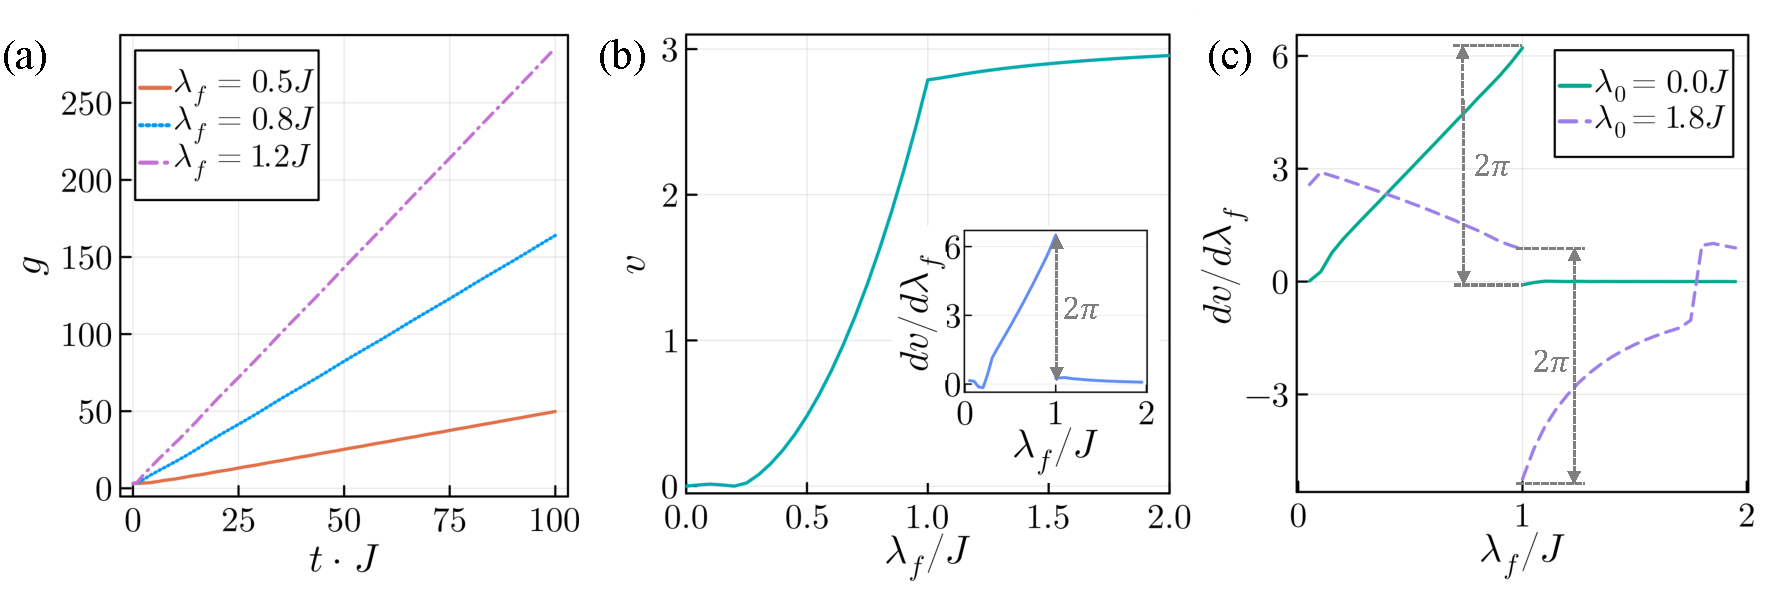
\includegraphics[width=1\textwidth]{figures/QV_1D_kitaev.pdf}
				\centering
				\bicaption{(a) 一维Kitaev模型从相同的初态$\lambda_0=0.2J$淬火到不同的$\lambda_f$对应的哈密顿量下量子态体积 $g(t)$随时间的演化。
					(b) 增长率$v$与不同$\lambda_f$之间的关系。内页是增长率$v$关于$\lambda_f$的导数,其在量子临界点处展现出了普适的跳变值$2\pi$。
					(c) 从不同$\lambda_0$对应的初态出发,$dv/d\lambda_f$随着$\lambda_f$的变化关系,且在 $\lambda_f=J$展现出了相同跳变值$2\pi$。}
					{(a) Quantum state volume $g(t)$ for the 1D Kitaev model in the quantum quench dynamics starting from the same initial states with $\lambda_0=0.2J$, but evolving under the Hamiltonian with different $\lambda_f$.
					(b) The growth velocity $v$ as a function of $\lambda_f$. The inset is its derivative with respect to $\lambda_f$ , which exhibits a discontinuity with an universal jump value $2\pi$.
					(c) $dv/d\lambda_f$ as a function of $\lambda_f$ starting from initial states with different $\lambda_0$, which share the same jump value of $2\pi$ at $\lambda_f=J$.}
				\label{fig:QV_1D_kitaev}
			\end{figure}
		
			第二个一维的例子是Su-Schrieffer-Heeger~(SSH)模型,它的哈密顿量是
			\begin{equation}
				H = \lambda\sum_{i=1}^{N}{c^\dagger_{i,A}c_{i,B}} + J\sum_{i=1}^{N}{c^\dagger_{i+1,A}c_{i,B}} + h.c.
			\end{equation}
			其中$i$是元胞的指标,每个元胞包含了A和B两种不同的格点。
			我们选择周期边界条件$c^\dagger_{N+1,A/B} = c^\dagger_{1,A/B}$之后,就可以通过傅里叶变换得到动量空间下的哈密顿矢量为$\vec{h}_k = (\lambda+J\cos{k},J\sin{k},0)$,其中第一布里渊区的范围是$k \in [0,2\pi)$。
			不失一般性地,我们考虑$\lambda > 0$且$J > 0$,于是哈密顿矢量被约化为$\vec{h}_k = (\lambda,Jk,0)$。
			当$\lambda_c=J$且$k_c=\pi$时,能隙闭合。
			我们从数值上检验了$C_1 = 2\pi$,如图~\ref{Fig:QV_1D_SSH}~(a)所示,并且这个结果对于不同的$\lambda_0$都是成立的,如图~\ref{Fig:QV_1D_SSH}~(b)所示。
			
			\begin{figure}[!htp]
				\centering
				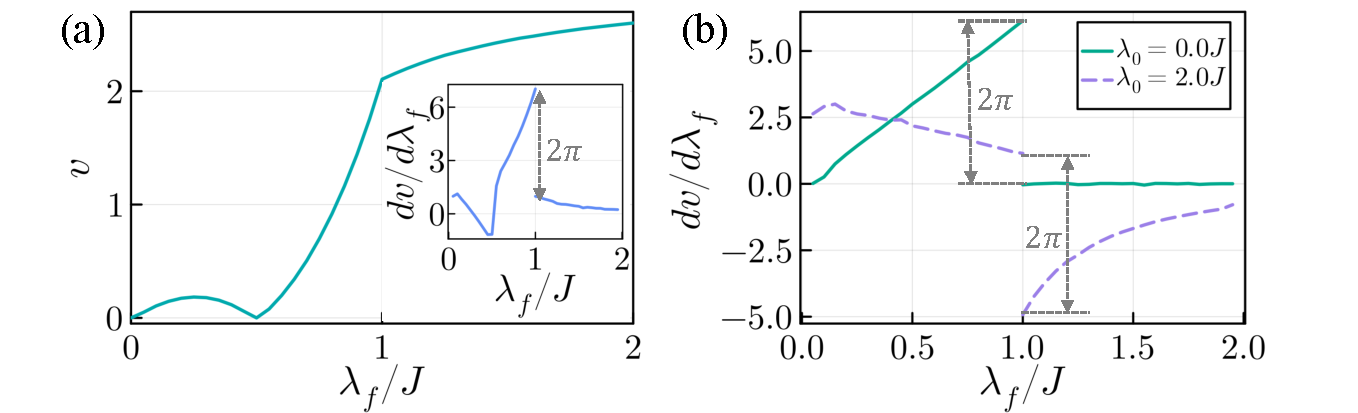
\includegraphics[width=1\textwidth]{figures/QV_1D_SSH.pdf}
				\centering
				\bicaption{(a) 当$\lambda_0 = 0.5J$时,线性增长的斜率随着$\lambda_f$的变化关系,并在$\lambda_f = 1.0J$处呈现出弯折。
					(b) 不同$\lambda_0$的跳变示意图,跳变值均为$2\pi$。}
				{(a) When $\lambda_0 = 0.5J$, the slope of linear growth with respect to $\lambda_f$, which exhibits a kink at $\lambda_f = 1.0J$.
					Inset: The derivative of the main set over $\lambda_f$, showing that the jump of slope at $\lambda_f = 1.0J$ equals $2\pi$.
					(b) The illustration of slope jumps at different $\lambda_0$, which all are equivalent to $2\pi$.}
				\label{Fig:QV_1D_SSH}
			\end{figure}
			
			最后一个一维的例子是带有周期交错化学势的费米子格点模型,它的哈密顿量是
			\begin{equation}
				H = -J\sum_{i=1}^{N}{c^\dagger_{i}c_{i+1}} + h.c. + (-1)^i\lambda\sum_{i=1}^{N}{c^\dagger_{i}c_{i}}
			\end{equation}
			考虑周期边界条件$c^\dagger_{N+1} = c^\dagger_{1}$之后,可以通过傅里叶变换得到动量空间的哈密顿矢量为$\vec{h}_k = (\lambda,0,2J\cos{k})$,其中第一布里渊区的范围是$k \in [0,\pi]$。
			不失一般性地,我们考虑$J > 0$,于是哈密顿矢量可以被约化为$\vec{h}_k = (\lambda,0,-2Jk)$。
			当$\lambda_c=0$且$k_c=\pi/2$,系统的能隙闭合。
			我们从数值上验证了$C_1 = 2\pi$,如图~\ref{Fig:QV_1D_AB}~(a)所示,结论对于不同的$\lambda_0$都是成立的,如图~\ref{Fig:QV_1D_AB}~(b)所示。
			
			\begin{figure}[!htp]
				\centering
				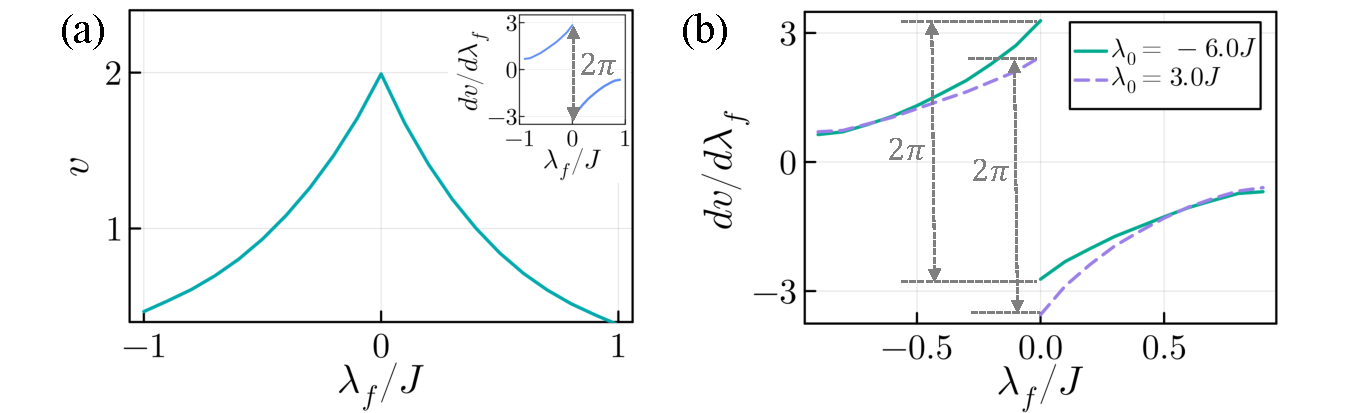
\includegraphics[width=1\textwidth]{figures/QV_1D_AB.pdf}
				\centering
				\bicaption{(a) 当$\lambda_0 = 10J$时,线性增长的斜率随着$\lambda_f$的变化关系,并在$\lambda_f = 0.0J$处呈现出弯折。
					(b) 不同$\lambda_0$的跳变示意图,跳变值均为$2\pi$。}
				{(a) When $\lambda_0 = 10.0J$, the slope of linear growth with respect to $\lambda_f$, which exhibits a kink at $\lambda_f = 0.0J$.
					Inset: The derivative of the main set over $\lambda_f$, showing that the jump of slope at $\lambda_f = 0.0J$ equals $2\pi$.
					(b) The illustration of slope jumps at different $\lambda_0$, which all are equivalent to $2\pi$.}
				\label{Fig:QV_1D_AB}
			\end{figure}
		
			对于二维的情形,我们也对两个不同的模型进行了计算。
			第一个模型是Qi-Wu-Zhang (QWZ)模型~\cite{Qi2006},它的哈密顿量是
			\begin{equation}
				\vec{h}_{QWZ}(\mathbf{k}) = [J\sin k_x, J\sin k_y, J(\cos k_x + \cos k_y) + \lambda(t)],\label{eq:QWZ}
			\end{equation}
			其中第一布里渊区的范围是$(k_x, k_y) \in (-\pi, \pi]$。
			这个模型分别在$\lambda = 0, \pm2J$处展现出了量子相变。
			对于$\lambda = 0$的情况,第一布里渊区内有两个能隙闭合点,即$\mathcal{N}=2$:$\mathbf{k}_c^1=(0,\pi)$和$\mathbf{k}_c^2=(\pi,0)$;
			而对于$\lambda = 2J(-2J)$的情况,第一布里渊区内就只有一个能隙闭合点,即$\mathcal{N}=1$,位于$\mathbf{k}_c=(0,0)$ ($\mathbf{k}_c=(\pi,\pi)$)。
			我们从公式\eqref{eq:QWZ}所描述的哈密顿量在控制参数$\lambda = \lambda_0$下的基态出发,然后突然将控制参数调节到$\lambda_f$,再让系统在这个新哈密顿量下演化,研究量子态体积$g(t)$的淬火动力学。
			$g(t)$依旧展现出了随时间的线性增长,如图~\ref{Fig:QV_2D_QWZ}~(a)所示。
			然后我们得到增长率$v(\lambda_f)$关于$\lambda_f$的导数。
			图~\ref{Fig:QV_2D_QWZ}~(b)和(c)说明了在$\lambda_f=-2J$和$\lambda_f=0$处分别出现了普适的跳变值,分别对应$\mathcal{N}=1$和$\mathcal{N}=2$的情形,与公式~\eqref{eq:Cd}中给出的结论$C_2 = 8$是一致的。
			
			\begin{figure}[!htp]
				\centering
				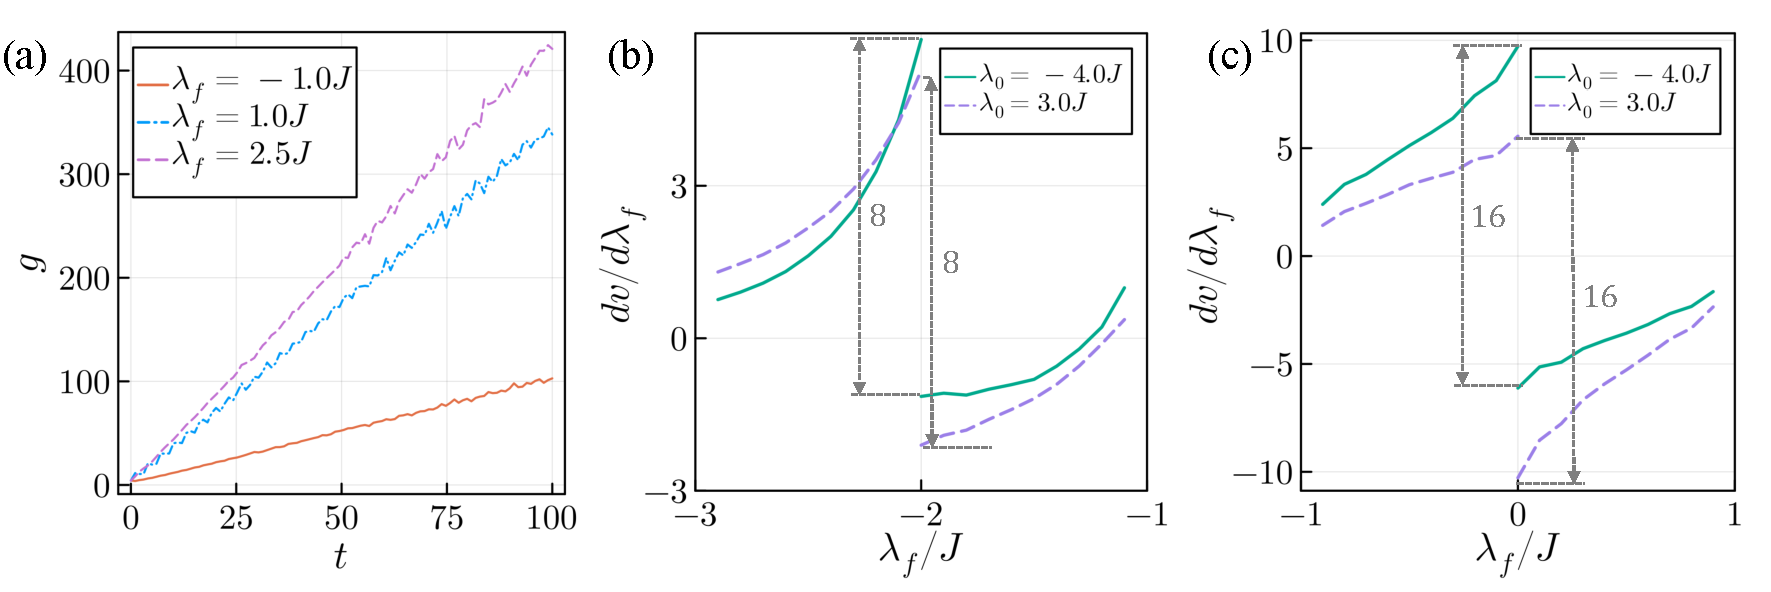
\includegraphics[width=1\textwidth]{figures/QV_2D_QWZ.pdf}
				\centering
				\bicaption{(a) 二维Qi-Wu-Zhang模型从相同的初态$\lambda_0=-0.5J$出发,在不同的哈密顿量$\lambda_f$下量子态体积的淬火动力学
					(b)和(c) $dv/d\lambda_f$随着$\lambda_f$在不同量子相变点(b) $\lambda_f=-2J$和(c) $\lambda_f=0$处的变化。
					$\lambda_f=-2J$ ($\lambda_f=0$)时,第一布里渊区内量子临界点的个数分别为$\mathcal{N}=1$ ($\mathcal{N}=2$)。}
				{(a) Quantum volume $g(t)$ for the 2D Qi-Wu-Zhang model in the quantum quench dynamics starting from the same initial states with $\lambda_0=-0.5J$, but evolving under the Hamiltonian with different $\lambda_f$.
					(b) and (c) $dv/d\lambda_f$ as a function of $\lambda_f$ around the different quantum critical points at (b) $\lambda_f=-2J$ and (c) $\lambda_f=0$.  The number of the gap closing points in the 1st BZ is $\mathcal{N}=1$ ($\mathcal{N}=2$) for the critical point at $\lambda_f=-2J$ ($\lambda_f=0$).}
				\label{Fig:QV_2D_QWZ}
			\end{figure}
		
	\section{结论与展望}
		总之,我们展示了量子临界性可以掌控远离基态的非平衡动力学,并诱导出普适的动力学行为。
		尽管量子体积依赖于无相互作用的能带结构,但其普适的速度跳跃完全由能隙闭合点附近的k渐近行为局部决定。
		因此,我们预期这种体积概念可以推广到存在相互作用的体系\cite{Souza2000},只要这些体系在临界点附近允许具有涌现平移对称性的有效场论描述,例如狄拉克物理和其他共形场论\cite{Francesco:2012aa,Wehling:2014aa}。
		而这正是在低维系统中普遍存在的特征\cite{Gogolin:2004aa}。
	
	
	